\section{Plan for completion}\label{sec:plan}
The development of new audio visualisations will start by targeting a specific
use case (see Section~\ref{sec:planusecase}) in selecting or extracting sets of
existing audio features (see Section~\ref{sec:planfeatsexist}), developing sets
of new audio features (see Section~\ref{sec:planfeatsnew}), then mapping those
features to visual properties including colour and texture (see
Section~\ref{sec:planvismap}). The development stage will make frequent use of
online testing (see Section~\ref{sec:planonline}) and intermittent use of
ethnographic testing (see Section~\ref{sec:planethno}) in evaluating and honing
the designs. Once successful visualizations have been developed for specific
use cases, attempts will be made at creating either an all-purpose or adaptive
audio visualization that can cope with all radio content (see
Section~\ref{sec:planall}).

The steps in the plan and deliverables are listed in
Section~\ref{sec:plandeliver} and the timetable is listed in
Section~\ref{sec:plantime}.

\subsection{Target use case}\label{sec:planusecase}
Due to the significant challenge of creating an all-purpose audio
visualization, this research will start by targeting use cases related to
popular radio production tasks.

\paragraph{Speech/music discrimination}
This is at the top of the classification hierarchy when it comes to radio
content, making it the simplest and most obvious use case to tackle. For this
reason, it was chosen for the first study where it was shown to be very
effective, even when using a very basic algorithm.

Further development of the SMD algorithm using the same approach as the first
study would be very difficult, as the difference in performance between the
algorithms would be marginal. The study was good at showing differences between
whole visualization systems of different designs in a realistic context (i.e.
is a SMD-enhanced waveform better than a non-enhanced waveform). However, the
study is not designed to pick out minor differences.

It may be possible to find edge cases where the algorithms start to fail, but
these would have to be chosen with great care so as not to bias the result. A
more successful path may be to do something similar to Tsiros
\cite{Tsiros2014}, where a short audio clip is played with its accompanying
visualization and participants are asked to rate how similar they are.

\paragraph{Speaker diarization}
Alternatively, a more challenging use case could be selected such as speaker
diarization, where a speech recording is segmented by where different people
are speaking. Rather than the output being binary (music/speech), the
visualization would have to map the sound of people's voices in such a way that
their individual contributions in the recording could be seen.

Although this is a more difficult use case, it is arguably more valuable
because of the significant amount of speech-based content that is produced.

\subsection{Feature development}\label{sec:planfeats}

\subsubsection{Existing features}\label{sec:planfeatsexist}
The literature review in Section~\ref{sec:litreviewfeats} shows that
speech/music discrimination and speaker diarization are popular research topics
that successful use many hand-crafted audio features. The study detailed in
Section~\ref{sec:study} found that for speech/music discrimination, mapping one
of these scalar features to a colour made a significant impact.

Attempting to map all of these features to a single visualisation will most
likely result in the user being overwhelmed with information. Success is much
more likely if a select few features are chosen/created which together can
fully distinguish the audio in the target use case.

There are many procedural methods available for taking a large set of features
and reducing them down to a smaller set, as detailed in
Section~\ref{sec:litreviewgeneration}. The algorithms can be separated into
feature selection, where a smaller set of individual features are chosen from
the larger set, and feature extraction, where all of the features are mapped to
a new smaller set of features. These can be further divided into unsupervised
methods, where nothing about the audio is known, and supervised methods, where
the audio is labelled.

It is not known which style of feature reduction algorithm would work best in
the context of visualisation, nor which algorithm within those groups would
perform best. In order to answer these questions, the project will start by
comparing unsupervised selection and extraction methods, before creating
labelled data sets to use in comparing supervised methods.

\subsubsection{New features}\label{sec:planfeatsnew}
Procedural methods of feature selection work to minimise correlation between
the output dimensions, but these may not necessarily work well for
visualization. It may be possible to develop a new set of features that do work
well for visualization, using what we know about the chosen use case and
audio-visual mappings.

Research into cross-modal links (see Section~\ref{sec:litreviewmodal}) has
identified a number of connections between the acoustic and visual properties
which could be used as the basis for development of new features. The
definition of the audio features shown to have strong mappings (e.g. pitch) do
not have very strict definitions, so could be moulded to the chosen use case.
For example, for speaker diarization pitch could mean the fundamental frequency
of somebody's voiced speech, the frequencies of the formants or some
relationship between them.

Development of new features would involve reviewing the literature to a greater
depth and attempting to come up with algorithms that could extract the
properties of audio which map strongly to vision.

\subsection{Visualisation mapping}\label{sec:planvismap}

\subsubsection{Colour}
Mapping features to colour is the most obvious route to visualisation as it
can easily be integrated into waveforms. Section~\ref{sec:litreviewcolour}
contains many examples of how false colour has been used to display three
features at once, but they have all relied on mapping to the RGB colour model.

RGB mapping is extremely common as it based on additive colour theory and is
the same format that is used to produce coloured light in displays. However, by
looking at the frequency response of the cones that the human eye uses to
perceive colour (see Figure~\ref{fig:cones}), we can see that it is highly
non-linear.

\begin{figure}[ht]
  \centering
  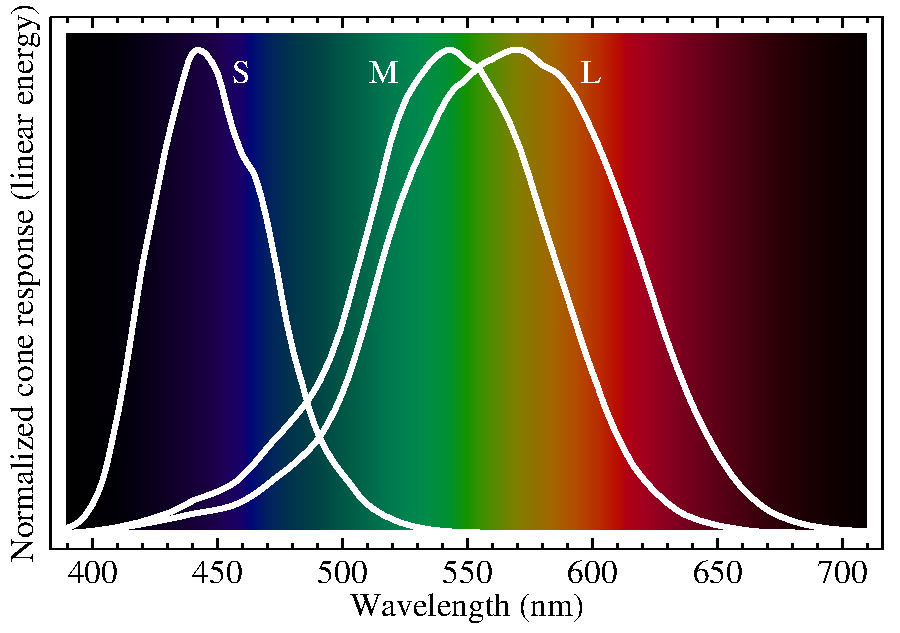
\includegraphics[width=0.5\textwidth]{figs/cones.pdf}
  \caption{Normalised response spectra of the three human cones (S, M and L).
    Image by BenRG. Licensed under Public domain via Wikimedia Commons.}
  \label{fig:cones}
\end{figure}

There are a variety of other colour models available which approach colour
representation from different angles, or map the RGB colour model to better
represent human perception of colour. The earliest colour model is CIE 1931
\cite{Smith1931}, which attempts to match the functions seen in
Figure~\ref{fig:cones}. CMYK (cyan, magenta, yellow, key/black) is based on a
subtractive colour model rather than the additive one used by RGB.  HSV (hue,
saturation, value) and HSL (hue, saturation, lightness) map the RGB colour
space so that the dimensions are better aligned to the attributes of colour as
perceived by human vision.  YUV is another method of encoding RGB which is made
up of one luminence and two chroma values. It is used in video encoding to
reduce the bandwidth of an image while maintaining as much perceptual
information as possible.

It is unknown which of these colour spaces is best suited for representing a
set of audio features and would be an interesting thing to test.

\subsubsection{Texture}
Texture and patterns occur everywhere in nature and can be used to distinguish
two items of the same colour.

Simple patterns, such as repeating lines, can easily be drawn using software.
Orientation, shape and spatial frequency are examples of three attributes that
have been shown to have a strong influence in visual search \cite{Wolfe2004}.
By generating textures that can map to such attributes, audio features could be
used to create textures that represent various acoustic properties.

Generation of texture using procedural methods is an existing area of research
\cite{Ebert1994} with successful applications in computer graphics. The aim of
the work is to design algorithms that create natural-looking textures (e.g.
wood grain, marble). The algorithms rely heavily on noise generation and
fractals to give the textures a natural feel, but ultimately the algorithms are
the result of a set of parameters. These parameters could be driven by a set of
audio features to create an audio visualization that looks much more natural.
When mapped to the right audio features, this could result in a high degree
of intuition.

Use of textures is an unexplored area for audio visualization, but could
potentially be an intuitive way of representing audio features.

\subsection{Evaluation}\label{sec:planeval}
Evaluation of audio visualizations is a critical part of developing the
algorithms and designs that drive them, and assessing their impact to real
production environments.

\subsubsection{Online}\label{sec:planonline}
The results of the first study showed that online testing of audio interfaces
can produce significant results, so it would be wise to keep exploring this
method of evaluation. The online system is well-suited to testing of specific
parts of a design or algorithm and studies can be put together and evaluated
relatively quickly, assuming that people are willing to continue to contribute.

As mentioned in Section~\ref{sec:planusecase}, the evaluation used in the first
study has worked for testing different visualization systems but would need to
be adapted for use in fine-grained development of the same kind of systems.
Such a system may present participants with a short audio clip and a few
candidate visualization. They would then be asked to select the one that most
closely matches, or rate them on their similarity to the audio.

\subsubsection{Ethnographic}\label{sec:planethno}
Online testing is useful for assessing different visualization designs in a
semi-controlled environment, but cannot fully evaluate the impact of a new
visualization in a real production environment. For this reason, online studies
will be used alongside ethnographic studies, which will consider how adding or
changing a visualization impacts producers in their day-to-day job.

BBC Redux is an online digital archive of previously-broadcast material (see
Section~\ref{sec:ingest}). Although not designed for use in production, this
valuable resource is often used by staff to find content for programmes. The
system is currently going through a significant upgrade of both its frontend
and backend, which will make it possible to integrate audio analysis
technology. By creating a development version of Redux, visualizations could be
added in to the existing service in a way that complements what is an existing
production tool. This could then be used as a testing platform to see how
production is affected by the introduction of new visualizations.

This work would be done using a series of existing user evaluation techniques.
Direct observation would involve sitting alongside a producer as they go about
their job and making notes about their behaviour and how it changes in relation
to the system under study. This can be enhanced by asking the producer in
question to chat about their thought process during this process (known as
think-aloud protocol) or conducting a semi-structured interview before and
after using the system.

As Redux contains a vast amount of content ($>$7 years for each TV and radio
station), it would be unfeasible to process all of it for such an experiment.
For this reason, the subjects for the study would have to be selected so that
their job only requires them to access a narrow range of dates, or narrow range
of programmes. Loftus Media is an independent production company that is
employed by the BBC to produce a radio programme based on the best bits of
other programmes in the past week. In this instance, it would be feasible to
process the past week of content for the purposes of testing a new
visualization. A study of this kind will rely on recruiting a production team
that work within such constraints.

\subsection{All-purpose visualization}\label{sec:planall}
Most of the research in this project will focus on specific use cases in order
to increase the likelihood of producing effective and useful visualizations.
However in the longer term, rather than having a handful of task-specific
visualizations, it would be better to produce a single visualization that
caters for all types of content. This could either be done using a fixed set of
features and visual mapping, or using a set of visualizations that are
automatically chosen based on the input content.

It would seem unfeasible to create an all-purpose visualization that is
intuitive to understand but can describe all types of content, so the work on a
general visualization would involve an aspect of training.  It is possible,
over time, to learn complex associations between vision and audition, as was
proved by Prof. Victor Zue \cite{Zue1986} who taught himself to read
spectrograms of speech recordings. However, this approach takes significant
time and effort.  Can a visualization be created to achieve something similar,
but with less training time? In the context of radio production, this could be
tested by performing a typical task using several different visualization,
after undergoing a set period of training for each.

Something similar could also be achieved by creating a set of various
task-specific visualizations and automatically selecting one of them depending
on the type of content being used. To give a simple example, if there is music
present in the audio recording, a speech/music discrimination visualization is
displayed, otherwise a speaker diarization visualization is shown. This
approach would require the definition and development of a variety of
visualization covering all types of content and tasks, in addition to a
classification stage which analyses the audio content and selects one of the
visualizations.

\subsection{Deliverables}\label{sec:plandeliver}
The work mentioned above has been grouped into a number of experiments which
are described and mapped out below:

\subsubsection{Experiment 1}
Develop a simple speech/music discrimination visualization and compare it using
an online test to a normal waveform and no waveform. (see results in
Section~\ref{sec:study}).

\paragraph{Deliverable}
Poster presentation at NordiCHI 2014

\subsubsection{Experiment 2}
Use unsupervised and supervised feature selection and extraction algorithms to
generate 3-dimensional feature vectors from commonly-used SMD and speaker
diarization features. Use these vectors as inputs to various colour models and
find the best combination for each use case using an online study.

\paragraph{Deliverable}
Conference paper at AES European Convention 2015

\subsubsection{Experiment 3}
Develop new features for SMD and speaker diarization. Use these features
and the best performing selected features as inputs to colour models and
texture generators and find the best combination using an online study.

\paragraph{Deliverable}
Conference paper at CHI 2016

\subsubsection{Experiment 4}
Using the results from experiments 2 and 3, integrate the best performing
visualization into an existing production tool. Recruit a production team to
take part in a study where the enhanced tool is used as part of their job and
their experiences are recorded and analysed.

\paragraph{Deliverable}
IEEE journal paper covering work to date

\subsubsection{Experiment 5}
Develop all-purpose audio visualisation with either fixed or adaptive mapping
using knowledge of audio features and cross-modal links. Test using large
online study.

\begin{landscape}
\subsection{Timetable}\label{sec:plantime}
\begin{ganttchart}[hgrid,vgrid,y unit chart=0.4cm]{1}{32}
\gantttitle{2014}{11}
\gantttitle{2015}{12}
\gantttitle{2016}{9} \\
\gantttitlelist{2,...,12}{1}
\gantttitlelist{1,...,12}{1}
\gantttitlelist{1,...,9}{1} \\
%
\ganttgroup{Experiment 1}{1}{7} \\
%\ganttbar{Ground truth data creation}{1}{2} \\
%\ganttbar{Develop plugin framework}{1}{1} \\
%\ganttbar{SMD visualisations}{2}{4} \\
%\ganttbar{Develop test platform}{3}{4} \\
%\ganttbar{User testing}{5}{5} \\
%\ganttbar{Results analysis}{6}{7} \\
\ganttbar{Write-up}{7}{7} \\
\ganttmilestone{Poster submission}{7} \\
%\ganttbar{Stage 1 write-up}{5}{5} \\
\ganttmilestone{Stage 1}{6} \\
%\ganttlink{elem2}{elem3}
%\ganttlink{elem4}{elem5}
%\ganttlink{elem5}{elem6}
%\ganttlink{elem7}{elem8}
%\ganttlink{elem9}{elem10}
%
\ganttgroup{Experiment 2}{8}{12} \\
\ganttbar{Feature selection/colour mapping}{8}{10} \\
\ganttbar{Testing and analysis}{11}{11} \\
\ganttbar{Write-up}{12}{12} \\
\ganttmilestone{Conference submission}{12} \\
%
\ganttgroup{Experiment 3}{13}{18} \\
\ganttbar{Feature development}{13}{14} \\
\ganttbar{Texture generation}{15}{15} \\
\ganttbar{Testing and analysis}{17}{17} \\
\ganttbar{Write-up}{18}{18} \\
\ganttmilestone{Conference submission}{18} \\
%
\ganttbar{Stage 2 write-up}{19}{20} \\
\ganttmilestone{Stage 2}{20} \\
%
\ganttgroup{Experiment 4}{21}{22} \\
\ganttbar{Real world integration}{21}{21} \\
\ganttbar{Ethnographic study}{22}{23} \\
\ganttbar{Write-up}{24}{24} \\
\ganttmilestone{Journal submission}{24} \\
%
\ganttgroup{Experiment 5}{25}{27} \\
\ganttbar{Adaptive visualisation dev}{25}{26} \\
\ganttbar{Testing and analysis}{27}{27} \\
%
\ganttbar{Thesis write-up}{28}{32} \\
\ganttmilestone{Thesis complete}{32} 
\end{ganttchart}
\end{landscape}
